\documentclass{article}

\usepackage[utf8]{inputenc}
\usepackage{amsthm}
\usepackage{amssymb}
\usepackage{mathtools}
\usepackage{graphicx}
\usepackage{mdframed}
\usepackage{float}
\usepackage[top=0.75in, bottom=0.75in, left=0.75in, right=0.75in]{geometry}
\usepackage{gauss}

\usepackage{array}
\allowdisplaybreaks

\makeatletter
\newcounter{elimination@steps}
\newcolumntype{R}[1]{>{\raggedleft\arraybackslash$}p{#1}<{$}}
\def\elimination@num@rights{}
\def\elimination@num@variables{}
\def\elimination@col@width{}
\newenvironment{elimination}[4][0]
{
    \setcounter{elimination@steps}{0}
    \def\elimination@num@rights{#1}
    \def\elimination@num@variables{#2}
    \def\elimination@col@width{#3}
    \renewcommand{\arraystretch}{#4}
    \start@align\@ne\st@rredtrue\m@ne
}
{
    \endalign
    \ignorespacesafterend
}
\newcommand{\step}[2]
{
    \ifnum\value{elimination@steps}>0\sim\quad\fi
    \left[
        \ifnum\elimination@num@rights>0
            \begin{array}
            {@{}*{\elimination@num@variables}{R{\elimination@col@width}}
            |@{}*{\elimination@num@rights}{R{\elimination@col@width}}}
        \else
            \begin{array}
            {@{}*{\elimination@num@variables}{R{\elimination@col@width}}}
        \fi
            #1
        \end{array}
    \right]
    & 
    \begin{array}{l}
        #2
    \end{array}
    \addtocounter{elimination@steps}{1}
}
\makeatother

\DeclarePairedDelimiter{\abs}{\lvert}{\rvert}
\DeclarePairedDelimiter{\norm}{\lvert \lvert}{\rvert \rvert}

\newtheoremstyle{break}% name
  {}%         Space above, empty = `usual value'
  {}%         Space below
  {\itshape}% Body font
  {}%         Indent amount (empty = no indent, \parindent = para indent)
  {\bfseries}% Thm head font
  {.}%        Punctuation after thm head
  {\newline}% Space after thm head: \newline = linebreak
  {}%         Thm head spec

\newtheorem{Def}{Definition}[section]

\theoremstyle{break}

\newtheorem{innerEx}{Exempel}[section]
\newtheorem{sats}{Sats}[section]
\newtheorem{Rem}{Anmärkning}[]

\newenvironment{Ex}
{\begin{mdframed} \begin{innerEx} \vspace{3pt}}
{\vspace{3pt} \end{innerEx} \end{mdframed}}  

\newenvironment{bevis}
{\begin{mdframed} \begin{proof} \vspace{3pt}}
{\vspace{3pt} \end{proof} \end{mdframed}}

\title{
	 Linjär Algebra\\
	 Föreläsning 4
    \author{Erik Sjöström}
}
\begin{document}
\maketitle

\section{Projektion} % (fold)
\label{sec:projektion}
\begin{Def}
    Låt $\vec{u}$ vara en vektor, och $L$ en linje med riktningsvektor $\vec{v}$. Den ortogonala projektionen $\vec{u_L}$ av $\vec{u}$ på $L$ är den vektor som det gäller att $\vec{u_L} \parallel \vec{v}$ och ($\vec{u}$ - $\vec{u_L}$) $\perp$ $\vec{v}$.
\end{Def}
\begin{center}
	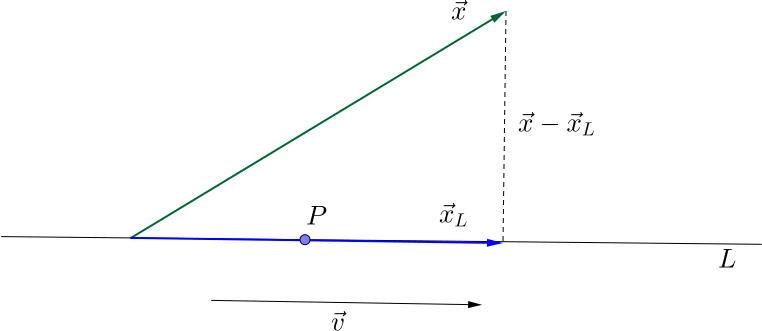
\includegraphics[scale=0.5]{projektion.png}
\end{center}
\begin{Ex}
    Låt:
    \begin{align*}
    &\vec{u} = \begin{bmatrix} 1\\3\\x \end{bmatrix} &\vec{v} = \begin{bmatrix} 3\\-3\\2 \end{bmatrix}
    \end{align*}
    Bestäm den ortogonala projektionen av $\vec{u}$ på linjen $L$ med riktningsvektor $\vec{v}$.\\
    Lösning: Vi vet att:
    \[
        \vec{u_L} = \frac{\vec{u} \cdot \vec{v}}{\norm{\vec{\vec{v}}}^2}
    \]
    Så nu gäller det bara att stoppa in värden:
    \begin{gather*}
    	\vec{u} \cdot \vec{v} = 1 \cdot 3 + 3 \cdot (-3) + x \cdot 2 = 2x - 6\\
    	\norm{\vec{v}}^2 = 3^2 + (-3)^2 + 2^2 = 22\\
    	\vec{u_L} = \frac{2x-6}{22} \cdot \begin{bmatrix} 3\\-3\\2 \end{bmatrix} = \frac{x-3}{11} \cdot \begin{bmatrix} 3\\-3\\2 \end{bmatrix}
    \end{gather*}
\end{Ex}
Vad blir $\vec{u} - \vec{u_L}$? (den del av $\vec{u}$ som är ortogonal mot $L$)
\[
    \vec{u} - \vec{u_L} = \vec{u}-\frac{\vec{u} \cdot \vec{v}}{\norm{\vec{v}}^2} \cdot \vec{v}
\]
\begin{Ex}
	\begin{align*}
    &\vec{u} = \begin{bmatrix} 1\\3\\0 \end{bmatrix} &\vec{v} = \begin{bmatrix} 3\\-3\\2 \end{bmatrix}
    \end{align*}
    Bestäm ortogonala komplementet av $\vec{u}$ på linjen $L$ med riktningsvektor $\vec{v}$\\
    Lösning:
    \begin{gather*}
    	\frac{\vec{u} \cdot \vec{v}}{\norm{\vec{v}}^2} \vec{v} = \frac{0-3}{11} \cdot \begin{bmatrix} 3\\-3\\2 \end{bmatrix} \\
    	\vec{u} - \frac{\vec{u} \cdot \vec{v}}{\norm{\vec{v}}^2} \vec{v} = \begin{bmatrix} 1\\3\\0 \end{bmatrix} + \frac{3}{11} \cdot \begin{bmatrix} 3\\-3\\2 \end{bmatrix} = \begin{bmatrix} 1 + \frac{9}{11}\\3- \frac{9}{11}\\\frac{6}{11}\end{bmatrix} = \frac{2}{11} \begin{bmatrix} 10\\12\\2 \end{bmatrix}
    \end{gather*}
    Denn vektor är ortogonal mot $L$.
\end{Ex}
Helt analogt definieras den ortogonala projektionen av vektorer på plan som:
\begin{Def}
    Den ortogonala projektionen $\vec{u_\pi}$ av vektor $\vec{u}$ på ett plan $\pi$ definieras som den vektor som ligger i planet och är sådan att $(\vec{u} - \vec{u_\pi}) \perp \pi$
    \begin{center}
    	\includegraphics[scale=0.5]{projektionplan.png}
    \end{center}
    \begin{Rem}
        Vektorn $\vec{u} - \vec{u_\pi}$ är parallell med planets normal
    \end{Rem}
\end{Def}
% section projektion (end)

\section{Avstånd mellan punkt och plan} % (fold)
\label{sec:avst_nd}
Givet en punkt P = (x,y,z), och ett plan $\pi : Ax + By + Cz =D$
\begin{Rem}
    Normalvektorn $\vec{n}$ = $\begin{bmatrix} A&B&C \end{bmatrix}$
\end{Rem}
\begin{center}
	\includegraphics[scale=0.5]{avstandplan.png}
\end{center}
Vi söker minsta avståndent $d$ mellan $P$ och $\pi$\\
\textbf{Härledning}:\\
Välj en punkt $Q$ i $\pi$ och bilda $\overrightarrow{QP}$ $d$ ges av den ortogonala projektionen av $\overrightarrow{QP}$ på normalen $\vec{n}$ till $\pi$.
\begin{gather*}
 	d = \frac{\abs{\overrightarrow{QP} \cdot \vec{n}}}{\norm{\vec{n}}} = \frac{\abs{P - Q} \cdot \vec{n}}{\norm{\vec{n}}} = \frac{\abs{P \cdot \vec{n} - Q \cdot \vec{n}}}{\norm{\vec{n}}}
 \end{gather*}
 Vi får att:
 \begin{gather*}
 	P \cdot \vec{n} = \begin{bmatrix} x&y&z \end{bmatrix} \begin{bmatrix} A\\B\\C \end{bmatrix} = Ax + By + Cz \\
 	Q \cdot \vec{n}: Q \in \pi \mbox{ om } Q = (x_0,y_0,z_0) \mbox{ så att } Q \cdot \vec{n} = D\\
 	\norm{\vec{n}} = \sqrt{A^2+B^2+C^2}
 \end{gather*}
 Vilket då ger oss:
 \[
     \frac{\abs{Ax+By+Cz-D}}{\sqrt{A^2+B^2+C^2}}
 \]
\begin{Ex}
    Bestäm avståndet $d$ från $P=(1,-4,-3)$ till planet $2x-3y+6z=-1$\\
    Lösning:
    \[
        d = \frac{\abs{2 \cdot 1 + (-r)(-4) + 6(-3) + 1}}{\sqrt{2^2 + (-3)^2 + 6^2}} = \frac{\abs{-3}}{7} = \frac{3}{7}
    \]
\end{Ex}

\section{Avstånd mellan punkt och linje} % (fold)
\label{sec:avst_nd_mellan_punkt_och_linje}
Givet en punkt P, en linje $L:x = P_0 + t \cdot \vec{v}$, där $\vec{v}$ är riktningsvektorn till $L$, $P_0$ är en punkt på $L$ och $t \in \mathbb{R}$\\
\textbf{Söker:} Minsta avståndet d mellan P och L\\
\textbf{Härledning:} Bilda vektor $\overrightarrow{P_0P}$. 
\begin{center}
	\includegraphics[scale=0.5]{avstandlinje.png}
\end{center}
Vi ser då at:
\[
    d = \norm{\overrightarrow{P_0P}} \cdot \sin(\alpha) = \frac{\norm{\overrightarrow{P_0P}} \cdot \norm{\vec{v}} \cdot \sin(\alpha)}{\norm{\vec{v}}} = \frac{\norm{\overrightarrow{P_0P} \times \vec{v}}}{\norm{\vec{v}}}
\]
\begin{Ex}
    Bestäm avståndet d från punkten $P=(3,-2,4)$ till linjen:
    \[
        L:x = \begin{bmatrix} -1\\1\\2 \end{bmatrix} + t \cdot \begin{bmatrix} 2\\1\\1 \end{bmatrix}, t \in \mathbb{R}
    \]
    Lösning:
    \begin{align*}
    	&\overrightarrow{P_0P} = \begin{bmatrix} 3\\-2\\4 \end{bmatrix} - \begin{bmatrix} -1\\1\\2 \end{bmatrix} = \begin{bmatrix} 4\\-3\\2 \end{bmatrix}\\
    	&\overrightarrow{P_0P} \times \vec{v} = \begin{bmatrix} -3 \cdot 1 - 2 \cdot 1\\2 \cdot 2 - 4 \cdot 1\\4 \cdot 1 - (-3) \cdot 2 \end{bmatrix}\\
    	&\norm{\overrightarrow{P_0P} \times \vec{v}} = \norm{\begin{bmatrix} -5\\0\\10 \end{bmatrix}} = \sqrt{25+0+100} = 5 \sqrt{5}\\
    	&\norm{\vec{v}} = \sqrt{2^2+1^2+1^2} = \sqrt{6}\\
    	&\mbox{Svar: } d = \frac{5\sqrt{5}}{\sqrt{6}} = 5 \sqrt{\frac{5}{6}}
    \end{align*}
\end{Ex}

% section avst_nd_mellan_punkt_och_linje (end)

% section avst_nd (end)

\section{Spegling} % (fold)
\label{sec:spegling_i_linje}
\begin{Def}
    Speglingen $\vec{u_s}$ av $\vec{u}$	 i en linje $L$ ges av:
    \[
        \vec{u_s} = 2 \vec{u_L} - \vec{u}
    \]
    Där $\vec{u_L}$ är den ortogonala projektionen av $\vec{u}$ på $L$.
    \begin{center}
    	\includegraphics[scale=0.5]{speglinglinje.png}
    \end{center}
\end{Def}
\begin{Def}
    Speglingen $\vec{u_s}$ av vektorn $\vec{u}$ i planet $\pi$ ges av:
    \[
        \vec{u_s} = 2 \vec{u_\pi} - \vec{u} 
    \]
    Där $\vec{u_\pi}$ är den ortogonala projektionen av $\vec{u}$ op $\pi$
    \begin{center}
    	\includegraphics[scale=0.5]{speglingplan.png}
    \end{center}
\end{Def}

\section{Matriser} % (fold)
\label{sec:matriser}
En matris är ett talschema med m rader och n kolumner, betecknas oftast som:
\[
    \begin{bmatrix} a_{11} &a_{12} &... &a_{1n}\\a_{21} &a_{22} &... &a_{2n}\\ \vdots &\vdots &\vdots &\vdots\\ a_{m1} &a_{m2} &... &a_{mn} \end{bmatrix}
\]
\begin{itemize}
	\item Sägs vara av typen/storleken $m \times n$
	\item $a_{ij}$ betecknar elementet på rad i, kolumn j
\end{itemize}
\begin{Ex}
    \[
        \mathbf{A} = \begin{bmatrix} 2&3&5\\-2&1&0 \end{bmatrix}
    \]
    \begin{itemize}
    	\item 
    	\item Är av typen $2 \times 3$
    	\item $a_{22} = 1$
    \end{itemize}
\end{Ex}
Ibland skriver man:
\[
    \begin{bmatrix} A = a_1&a_2&...&a_n \end{bmatrix}
\]
Vilket är kolumnvektorerna till matrisen A
\section{Räkneregler} % (fold)
\label{sec:r_kneregler}
Matrisadditionen $\mathbf{A} + \mathbf{B}$ definieras: Elementen i respektive kolumn adderas.
\begin{Rem}
    \textbf{A} och \textbf{B} måste vara av samma typ/storlek
\end{Rem}
\newpage
\begin{Ex}
    \begin{gather*}
    	\mathbf{A} = \begin{bmatrix} 1&0\\2&3 \end{bmatrix}, \mathbf{B} = \begin{bmatrix} 0&5\\5&1 \end{bmatrix}\\
    	\mathbf{A} + \mathbf{B} = \begin{bmatrix} 1&0\\2&3 \end{bmatrix} + \begin{bmatrix} 0&5\\5&1 \end{bmatrix} = \begin{bmatrix} 1&5\\7&4 \end{bmatrix}
    \end{gather*}
\end{Ex}

\noindent
Multiplikation med skalär: 
\begin{align*}
&k \cdot \mathbf{A} &k \in \mathbb{R}
\end{align*}
Alla elementen i \textbf{A} multipliceras med k.
\begin{Ex}
    k = 5, \textbf{A} som innan
    \[
        k \cdot \mathbf{A} = 5 \cdot \begin{bmatrix} 1&0\\2&3 \end{bmatrix} = \begin{bmatrix} 5&0\\10&15 \end{bmatrix}
    \]
\end{Ex}
Följande räkneregler gäller för matrisaddition respektive multiplikation med skalär:\\
Låt: \textbf{A}, \textbf{B}, \textbf{C} vara $m \times n$ matriser, och $r,s \in \mathbb{R}$
\begin{itemize}
	\item \textbf{A} + \textbf{B} = \textbf{B} + \textbf{A}
	\item (\textbf{A} + \textbf{B}) + \textbf{C} = \textbf{A} + (\textbf{B} + \textbf{C})
	\item \textbf{A} + $\mathbb{O}$ = \textbf{A}
	\item r $\cdot$ (\textbf{A} + \textbf{B}) = r $\cdot$ \textbf{A} + r $\cdot$ \textbf{B}
	\item (r + s) $\cdot$ \textbf{A} = r $\cdot$ \textbf{A} + s $\cdot$ \textbf{A}
	\item r $\cdot$ (s $\cdot$ \textbf{A}) = (r $\cdot$ s) $\cdot$ \textbf{A}
\end{itemize}
\begin{Rem}
    $\mathbb{O}$ är nollmatrisen, dvs den matris där alla element är 0.
\end{Rem}


% section r_kneregler (end)
% section matriser (end)
% section spegling_i_linje (end)
\end{document}
